\begin{figure}[h]
\centering
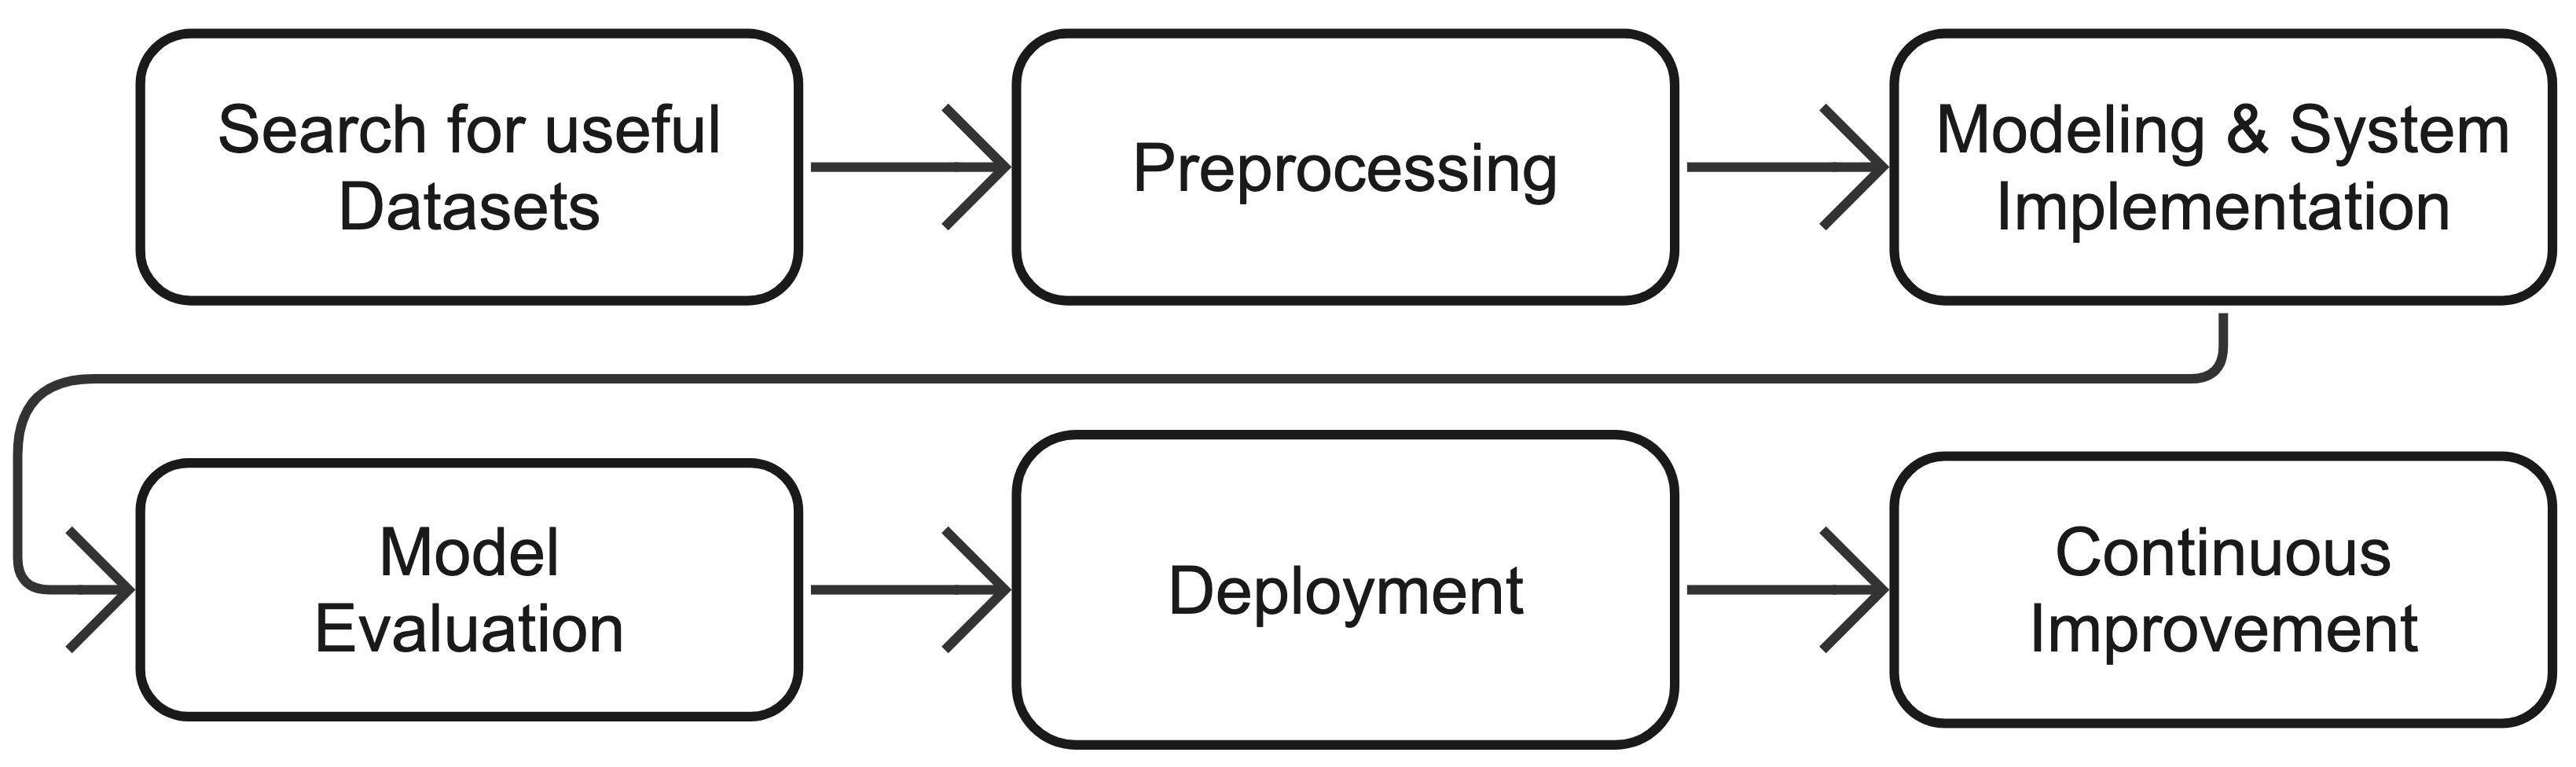
\includegraphics[width=\textwidth]{images/methodology2.png}
\caption{Methodology}\label{fig:methodology}
\end{figure}

\noindent 
%As seen in the previous section \acrshort{fer} and \acrshort{ser} is a relevant research area within various applications and fields. 
In this section, we will present the methodology for developing both a facial- and a speech emotion recognition system. Consequently, this section discusses the several methodical steps that need to be taken to address the research questions and reach the research goals.
%this section discusses several steps, for example data collection, preprocessing, modeling and model evaluation, including the user feedback. 


\begin{enumerate}
\color{blue}
    \item \textbf{Data Collection:}
    The first step in the project report is the data collection. This step is relevant, because the performance of emotion recognition models is highly dependent on the quality and diversity of the dataset used to train them. Therefore, it is necessary to collect a large and diverse dataset of both facial and speech emotional expressions to train and test the models. During the data collection process, the licence to use the corresponding data is considered.
    
    \item \textbf{Data Preprocessing:}
    Secondly comes the data preprocessing, which is crucial for cleaning and preparing the collected data for training the model. This step may involve data augmentation and feature extraction, depending on the specific techniques used for \acrshort{fer} and \acrshort{ser}. Data preprocessing is also essential for ensuring that the dataset is balanced and is a main step to ensure the model can generate good results.
    
    \item \textbf{Model and System Implementation:}
    The next crucial step is the implementation and training of the \acrshort{fer} and \acrshort{ser} models. Hereby, different machine learning frameworks may be used. Lastly, both models will be integrated into two individual pipelines that should be able to process real-time data streams and predict the according emotion of the user. 
    
    \item \textbf{Model Evaluation:}
    The model evaluation, which is the fourth phase, aids in determining how well the \acrshort{fer} and \acrshort{ser} models operate, utilizing evaluation criteria like accuracy, precision, and recall. Model evaluation is crucial for deciding which models are best suitable and for identifying any weaknesses or potential areas for improvement.
        
    \item \textbf{Deployment:}
    Thereafter, the final application will be deployed, whereby the \acrshort{fer} and \acrshort{ser} models will be integrated into a single system. Deployment is essential for testing the system's performance in real-world scenarios and verifying that the models can work together effectively and the feedback system works.
    
    \item \textbf{Continuous Improvement:}
    Lastly, the final step is a continuous improvement of the system. This involves continually updating and improving the \acrshort{fer} and \acrshort{ser} models e.g. through user feedback. This step may later also involve monitoring the system's performance, as well as adding new features and functionality to the system. Continuous improvement is essential for ensuring that the \acrshort{fer} and \acrshort{ser} models can adapt to new data and different real-world scenarios and can continue to perform well over time, which is according to our research goal. 
\end{enumerate}

\noindent By following these steps, we aim to develop a robust and accurate system that can recognize emotions from facial expressions and speech signals and can be used in various applications such as healthcare, marketing and security.



%\section{Facial Emotion Recognition}
%\begin{comment}
To Do:
\begin{itemize}
\color{red}
     \item Define the specific goals of the study, e.g., which characteristics of the problem will be used to assess the validity of the proposed solution?
     \item Design an empirical strategy to address the specific goals established.
    \item The pipeline implemented must be shown to work on a non-trivial (possibly real-world) example— a toy problem is not admitted.
    \item The pipeline implemented is experimented using a dataset with 3D images.
    \item A comprehensive analysis of multiple performance indicators.
    \item Implementation of the user feedback mechanism.
\end{itemize}

\begin{enumerate}
\color{blue}
\item \textbf{Preprocessing:} Explain the steps taken to preprocess the images, such as resizing, cropping, and normalization. Also, mention any techniques used to address issues like noise or distortion in the images.
\item \textbf{Feature Extraction:} Outline the techniques used to extract features from the images. This could include handcrafted features or deep learning approaches such as convolutional neural networks.
\item \textbf{Modeling:} Explain the algorithm used to build the model for emotional recognition in images, including any modifications made to the model architecture or hyperparameters.
\item \textbf{Evaluation:} Describe the evaluation metrics used to assess the performance of the model, such as accuracy, precision, recall, or F1-score. Also, mention the cross-validation approach used to ensure the generalization of the model.
\item \textbf{Comparison with Previous Studies:} Compare the results of your model with those of previous studies on emotional recognition in images, if any.
\item \textbf{Ethical Considerations:} Discuss the ethical considerations related to the use of image data, such as ensuring the privacy and confidentiality of the participants in the dataset.
\item \textbf{Limitations and Future Work:} Mention the limitations of your study and outline the future work that can be done to improve the emotional recognition in images.
\end{enumerate}
\end{comment}

\begin{figure}[h!]
\centering
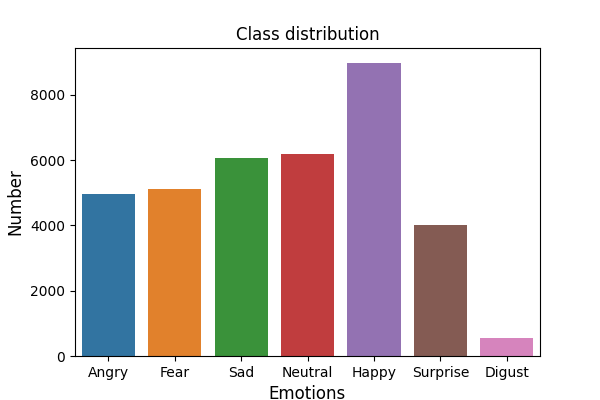
\includegraphics[scale=0.8]{barplot1.png}
\caption{Barplot of the distribution of the different classes of emotion.}\label{fig:emo-distribution}
\end{figure}

\begin{enumerate}
\item \textbf{Data Collection:} %The fer2013 dataset is handled according to the terms of the Open Database License (ODbL), which states the following: "The Licensor grants to You a worldwide, royalty-free, non-exclusive, perpetual, irrevocable copyright license to do any act that is restricted by copyright over anything within the Contents, whether in the original medium or any other. These rights explicitly include commercial use, and do not exclude any field of endeavour. These rights include, without limitation, the right to sublicense the work." \cite{odbl} We may use additional datasets provided by kaggle or other sources. 

To recognize emotions in images, the kaggle dataset \textbf{FER2013} \cite{FER2013} will be used. This dataset was prepared by Pierre-Luc Carrier and Aaron Courville as part of an ongoing research project and contains $35,887$ images, displaying the emotions anger, fear, sadness, neutralilty, happiness, surprise and disgust. Hereby, Figure \ref{fig:emo-distribution} represents the corresponding distribution of those emotions. Moreover, this dataset includes people from different genders, ethnicities and ages. Furthermore, the FER2013 dataset is handled according to the terms of the Open Database License (ODbL), which states the following: ``The Licensor grants to You a worldwide, royalty-free, non-exclusive, perpetual, irrevocable copyright license to do any act that is restricted by copyright over anything within the Contents, whether in the original medium or any other. These rights explicitly include commercial use, and do not exclude any field of endeavour [...].'' \cite{odbl} We may also use additional datasets provided by kaggle or other sources.

\begin{figure}[h]
\centering
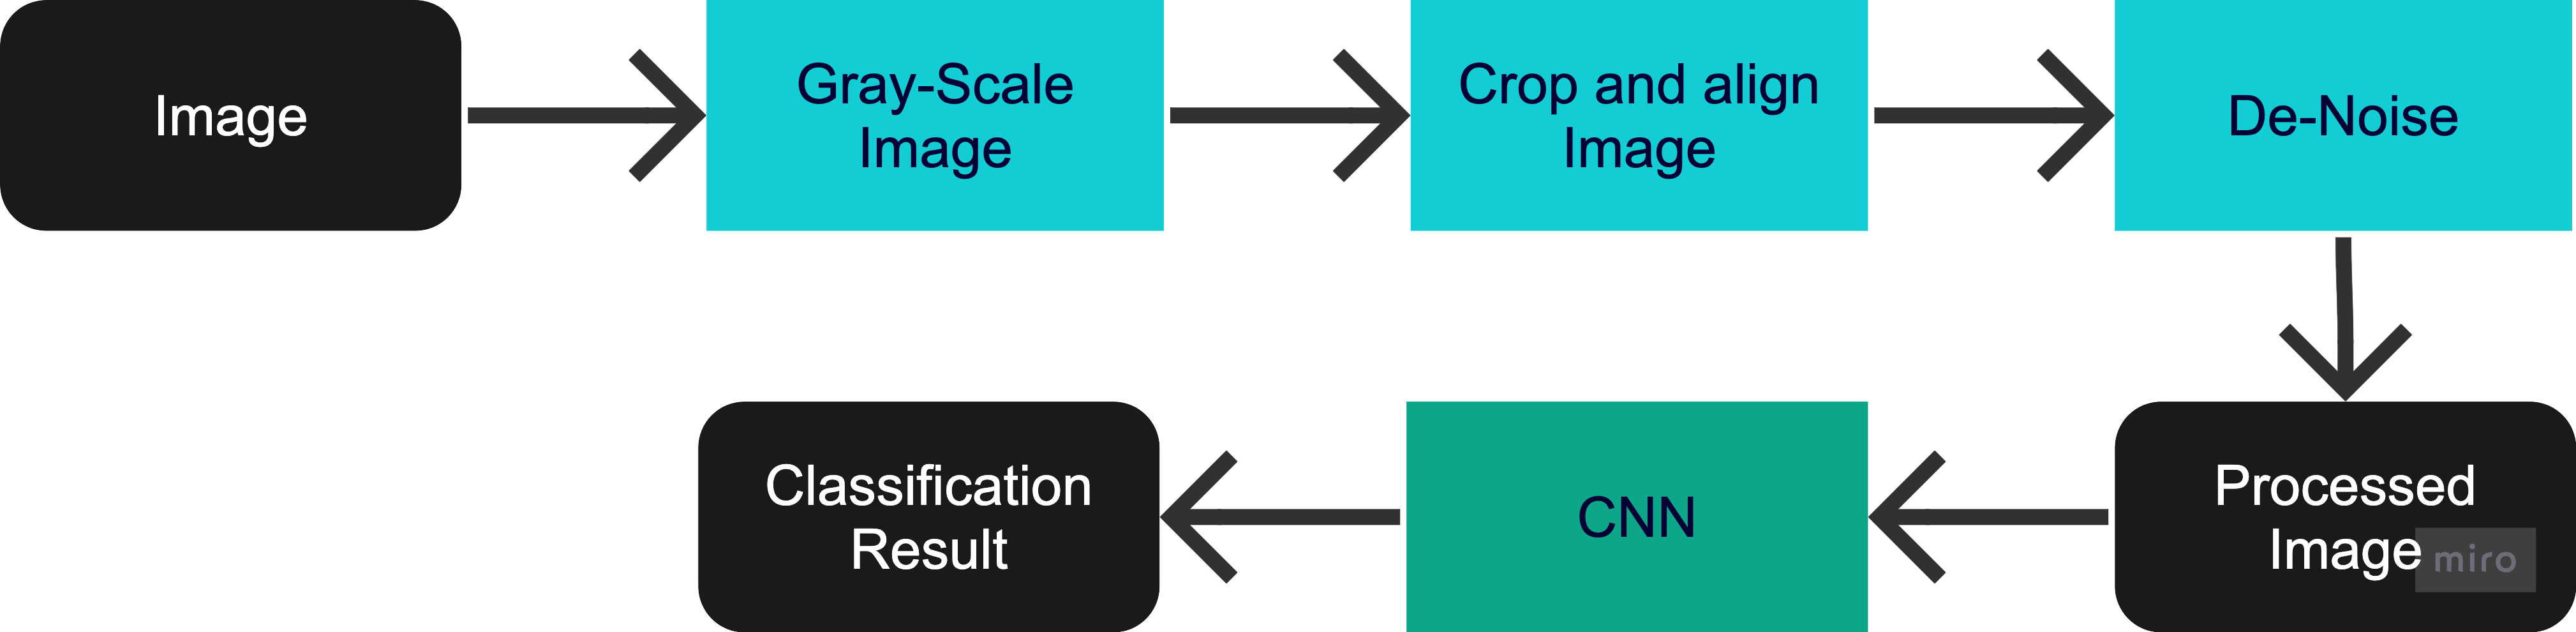
\includegraphics[width=0.9\textwidth]{images/fer-preprocessing-modelling.png}
\caption{Preprocessing and Modeling.}\label{fig:prep-mod}
\end{figure}

\item \textbf{Preprocessing:}
Before using the datasets, they will be preprocessed to exclude irrelevant images/emotions. Data preprocessing includes reducing different types of noises, resizing the picture, and aligning facial features. The method typically used to achieve the results is the eye selection method. Figure \ref{fig:emo-distribution} provides an example image of the different facial expressions with their corresponding labeled emotion. 
The \textit{FER2013} dataset provides preprocessed and labeled grayscaled images of facial emotions. We will however implement a pipeline to process new images. This will contain the following steps. The first step is to convert the (RGB) color image to a grayscale image. The colors in images can often contain clutter and hinder the model form detecting faces accurately. After the grayscale conversion, the next step is to crop and align the images, so that we are left only with the face. We should mention, that in this step we have to consider the resolution of the image and if the crop is still usable after the crop. The next step is to de-noise the image and apply filtering. De-noising the image will amplify and enhance the meaningful features of an image while reducing background noise.   Filtering is the process of altering properties of the image, for example contrast and saturation. For grayscaling and cropping the image we will use the OpenCV library.

\item \textbf{Modeling:}
Afterwards, a CNN with 2D convolutional layers will be used. This approach has been shown to be effective for image recognition tasks. We will experiment with the layers and parameters to try to achieve the best possible results. 

\begin{figure}[h]
\centering
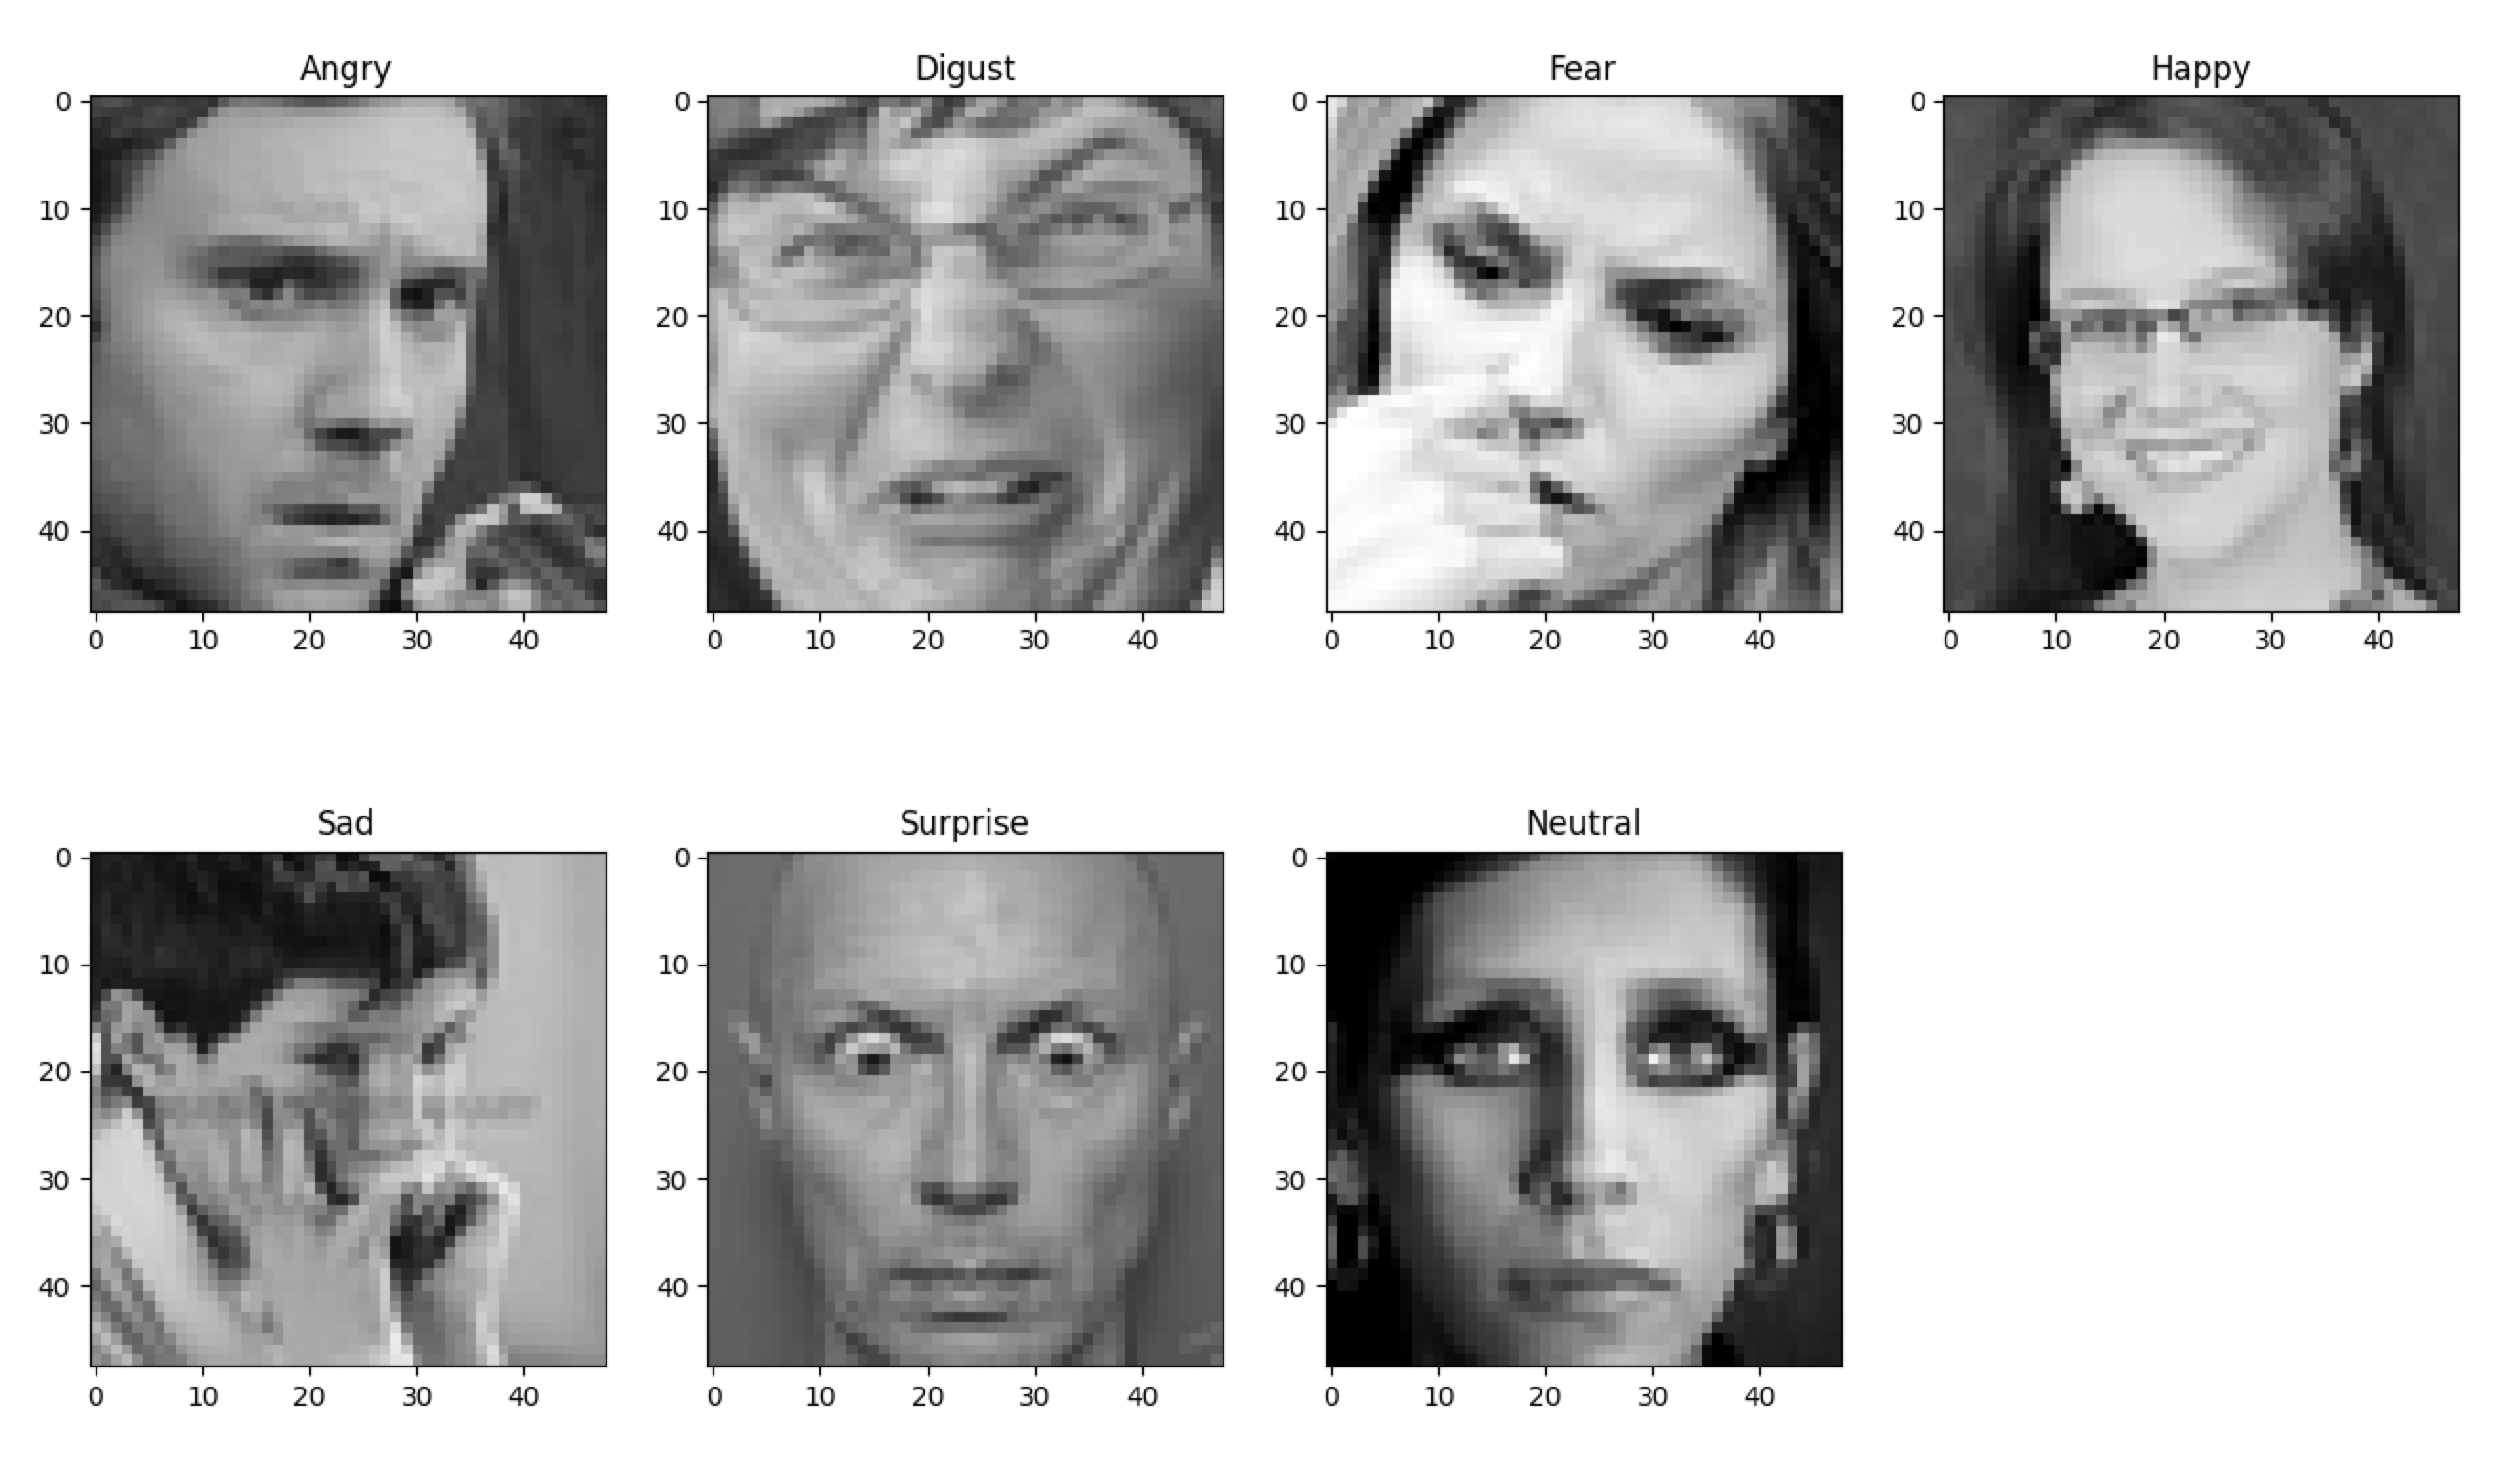
\includegraphics[width=0.9\textwidth]{faces1.png}\\
\caption{Facial expressions with corresponding emotions. \cite{FER2013}}\label{fig:faces}
\end{figure}

\newpage
\item \textbf{Model Evaluation:}
After training a model, the next goal is to test the model on new data. For this we can first use the test data and measure the accuracy, precision and recall. However for more practical applications our goal would be to implement an image preprocessing pipeline to allow us to apply the trained model on real-world captured images. This can then in turn be applied to frames of a video evaluating the emotions of one person (possibly multiple people if feasible). This will also preform as an alternative to the classic metrics for quality assurance, by allowing the person captured on the image to input their actual emotion and comparing their actual emotion to the predicted one. If we collect the new labeled images that were imputed by a user, we can retrain the model with more data, if the accuracy drops below a predetermined threshold.

\begin{figure}[h]
\centering
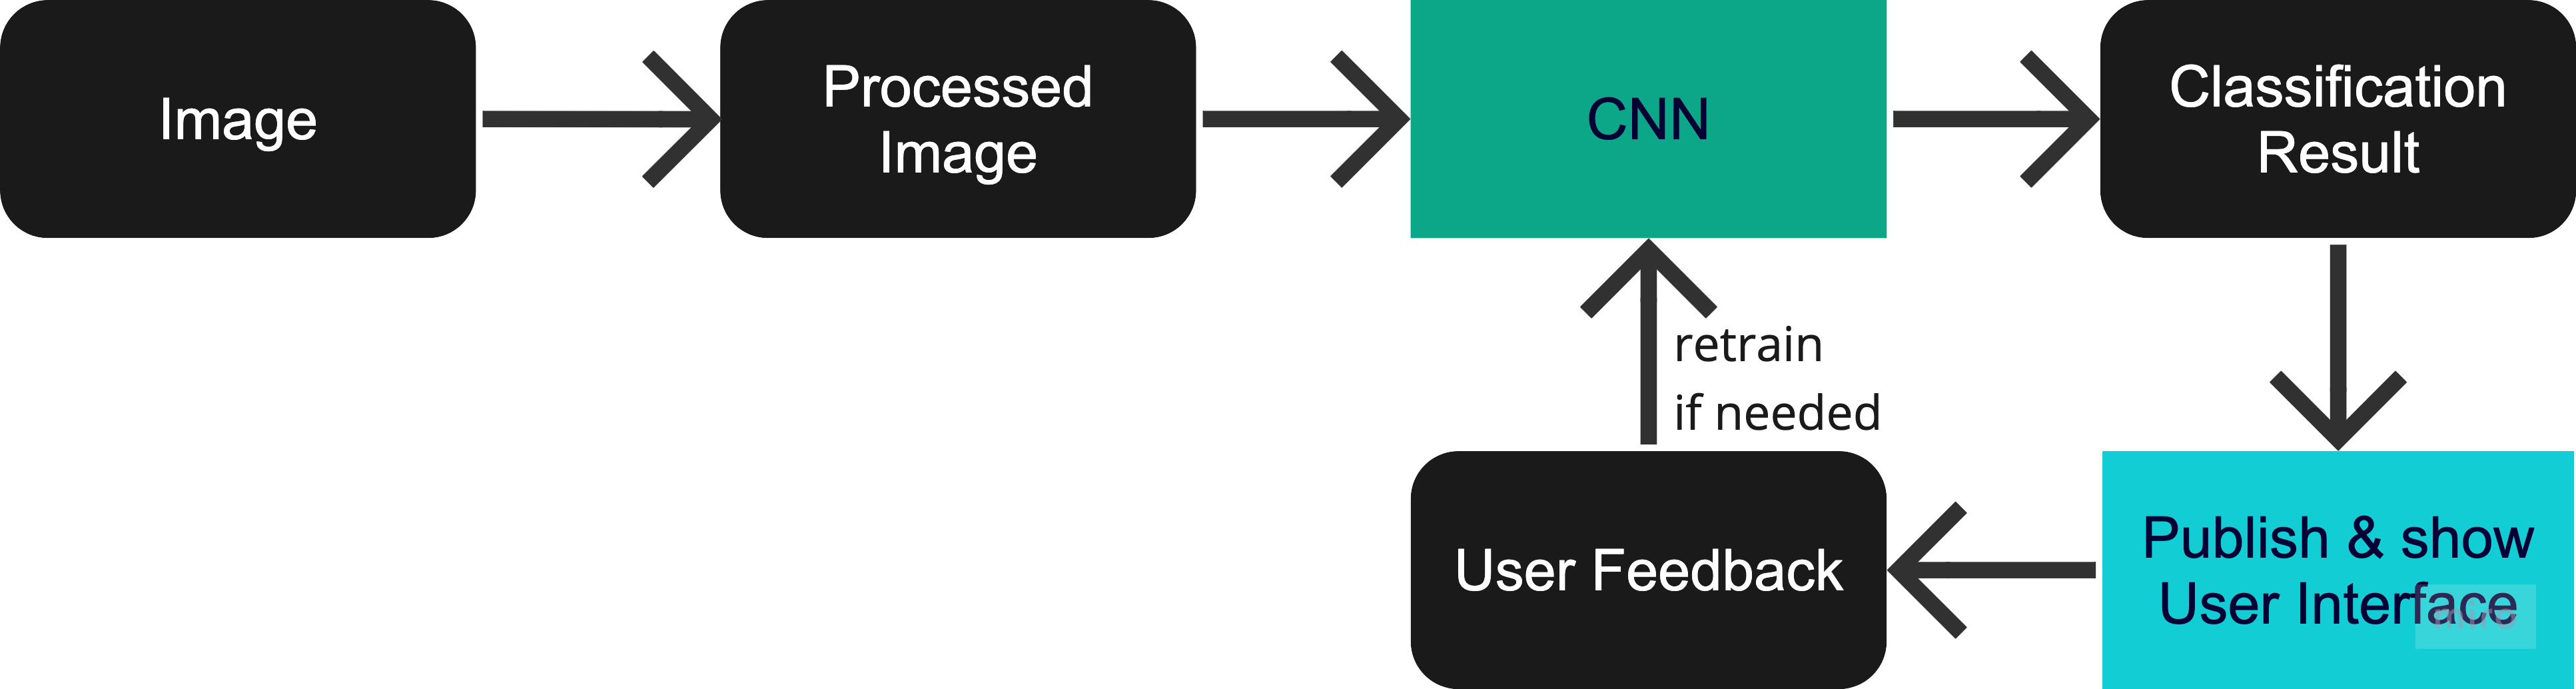
\includegraphics[width=0.9\textwidth]{images/fer-user-feedback.png}\\
\caption{General overview of the \acrshort{fer} system and user feedback}\label{fig:userfb}
\end{figure}

\end{enumerate}
\newpage

\begin{comment}
    \noindent We will implement the following files, containing classes for different models, data processing and tests: 
    \begin{enumerate}
        \item main.py
        \item ann\_model.py
        \item dataprocessing.py
        \item tests.py
    \end{enumerate}
    
    To address:
    \begin{itemize}
    \color{blue}
        \item Basic interface to better define the use case of the trained model. 
        \item Model Training: Train a deep neural network model using the preprocessed dataset.
        \item Model Evaluation: Evaluate the trained model using various metrics such as accuracy, precision, and recall.
        \item Get an Accuracy of around 65\% 
        \item System Development: Develop the emotional recognition system using the trained model and
        software engineering principles such as modular design, testing, and documentation.
        \item System Evaluation: Evaluate the developed system using various metrics such as performance, scalability, and maintainability.
        \item User Feedback: Incorporate user feedback mechanisms to improve the system’s accuracy and adaptability to new scenarios.
        \item Continuous datastreams (i.e. Video)
        \item Visualisation (Graphs, Barplots, ...) 
    \end{itemize}
\end{comment}

%\section{Preliminary results and findings}
%\section{Implications of the results}
%\section{Speech Emotion Recognition}
%\begin{enumerate}
\item \textbf{Data Collection:} \\
% Jana's task:
To train the model, we decided to use the crowd sourced CREMA-D data \cite{cremad} set that is downloadable from kaggle.com under the Open Data Commons Attribution License (ODC-By). This license allows to copy, distribute and use the database, furthermore to produce works from the database and to modify, transform and build upon it \cite{odc-by}.

The data set consists of 7,442 audio clips with the following characteristics: 
\begin{itemize}
    \item 12 different sentences
    \item six different emotions: Anger, Disgust, Fear, Happy, Neutral, Sad
    \item four different emotion levels: Low, Medium, High, Unspecified
    \item number of actors: 91
    \begin{itemize}
        \item age: ranging from 20 to 74 years
        \item ethnicity: African American, Asian, Caucasian, Hispanic, Unspecified
    \end{itemize}
\end{itemize}



\item \textbf{Preprocessing for Training:} \\
% Jana's task:
To increase the number and variety of data samples and to ensure robustness of the system to non-trivial scenarios, we will perform data augmentation in the form of random pitch shifts and time stretch transformations. Here, the python libraries Audiomentations and Librosa are useful. Both libraries are open-source and available for free. 

Then, we will calculate spectrograms from the raw audio samples by running a Fast Fourier Transform (FFT) algorithm. Here, again Librosa comes in handy. The spectrograms can then be fed into the neural networks.  

\begin{figure}[h]
\centering

\includegraphics[width=0.9\textwidth]{images/ser-preprocessing.png}\\
\caption{Preprocessing for Training.}\label{fig:ser_preprocessing}
\end{figure}

%\item \textbf{Feature Extraction:} 
\item \textbf{Modeling:} As already presented in chapter \ref{chap:project-ideas}, we are goint to use two different approaches for \acrshort{ser}, as is displayed in figure \ref{fig:ser_modeling}.\\
% Jana's task:
\emph{1. Approach: phonological information}

For the first approach, we will create a \acrfull{crnn},  i.e. a sequential neural network with 1D convolutional layers. It will take the spectrograms as input and outputs the most likely emotion associated with the input. Here, the python library Keras can be used to easily build a neural network by adding desired layers to the model. Keras is open-source and available for free. 

\emph{2. Approach: semantic information}

For the second approach, a combination of two neural networks will be used. First, an \acrfull{asr} model transforms the spectrograms into a textual representation of the utterance. This can again be done with Keras as it additionally offers APIs to pre-trained ASR models like DeepSpeech, an open-source model by Mozilla.
Then, the obtained text is assigned to an emotion by a transformer-based neural network. Here, the python library Hugging Face can be used. It is free, open-source and offers pre-trained transformer models like BERT. 
Since the ASR model and the transformer model are already pre-trained on a large corpus of data and our application scenario is kept general instead of domain-specific, it is not strictly necessary to find additional datasets for training the ASR model and the transformer model ourselves. \\

\begin{figure}[h!]
\centering
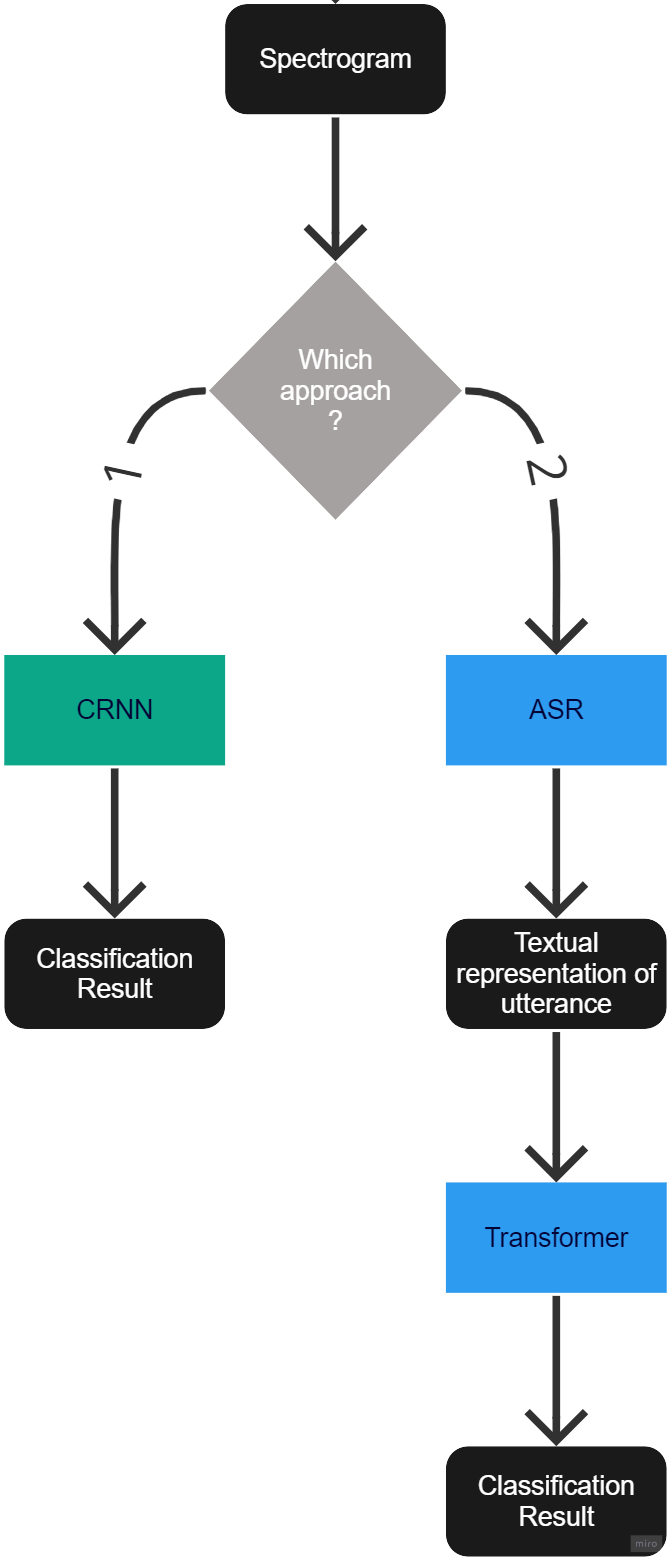
\includegraphics[scale=0.5]{images/SER_Modeling.png}\\
\caption{Modeling.}\label{fig:ser_modeling}
\end{figure}



\item \textbf{Model Evaluation:} \\
Test where we will run the model with a given input and compare its output with an expected output. The goal is to keep a track of the precision and loss of the model in training. The model must have a loss under a certain value and a precision above a certain value. During the development, we will also take advantage to unitary test for code coverage, these unitary tests will be needed to validate commit on the source control (GitHub in our case) of the project. Using this test will allow us to have an automated test pipeline that would be use for CI/CD. 

%Data splitting for Cross-Validation
%True positive (TP), True negatice (TN), False positive (FP), False negative (FN) when the model is not able to recognize any emotion.
%\begin{itemize}
%    \item Accuracy test,
%    By calculating how accurate is the model, using the following formula, $Accuracy = \frac{TP + TN}{N_{outputs}}$, we can test the success rate of the model.
%
%    \item Precision Test
%    Using the following formula, $Precision = \frac{TP}{TP + FP}$, we can test among the positive answers, the true positive rate.
%    
%    \item Sensitivity Test
%    $Sensitivity = \frac{TP}{TP + FN}$
%
%    \item Specificity Test
%    $Sensitivity = \frac{TN}{TN + FP}$
%    
%\end{itemize}

\color{black}
\item \textbf{System Development:} \\
% Jana's task
To test the speech emotion recognition in real-world scenarios, the trained neural networks will be embedded in a pipeline. 
The first step will be to record the users' utterances with a microphone. The continuous audio stream should then be cut every $x$ seconds to obtain the data samples. These will be preprocessed and fed into the neural networks. The results from both of the approaches will then be continuously published on the user interface. Here, the users indicate whether one or both of the classifications are correct and if not, what their actual emotion was. The user feedback will be stored along the respective audio sample and then used to retrain the models after the session. 
\color{blue}
%\item \textbf{System Evaluation:} including Comparison with Previous Studies: \\
% Ergi's task:
%The use of speech audio data in various applications has raised ethical considerations, particularly regarding the privacy and confidentiality of the participants in the dataset. Collecting audio data without the consent of the participants or disclosing the identity of the speakers can be a violation of privacy. Moreover, the use of audio data for purposes other than those that were originally intended can also result in ethical dilemmas. It is essential to ensure that the audio data collected is used only for legitimate purposes and that participants' personal information is kept confidential.
%\item \textbf{Limitations and Future Work:} \\
\end{enumerate}

%\section{Preliminary results and findings}
%\section{Implications of the results}